\section{Spineless Traversal}

Spineless Traversal improves on Double Dirty Bit
  by jumping directly between dirty nodes
  without accessing any auxiliary nodes;
  as a result, it suffers dramatically fewer cache misses.
Achieving this requires a more computationally heavy approach:
  storing all dirty nodes in a priority queue
  and maintaining the correct traversal order
  using an order maintenance data structure.
Spineless Traversal's savings in cache misses
  typically outweigh the greater computational requirements
  of these data structures.
Since Spineless Traversal is complex,
  this section develops it incrementally,
  first introducing the idea of a queue storing dirty nodes,
  then adding timestamps to maintain traversal order,
  and finally introducing the order maintenance structure
  to handle node insertion and deletion.
A final step optimizes bulk insertions and deletions.

\subsection{Jumping Directly to Dirty Nodes}

To jump directly to dirty nodes,
  we introduce a queue
  that stores pointers to dirty nodes.
More specifically, elements of the queue represent
  dirty bits in the layout tree that need to be cleared,
  and are represented in the queue by
  a pointer to the relevant layout node
  and an enumeration identifying
  which dirty bit needs to be cleared.
When a dirty bit is set,
  the corresponding node and enumeration are added to the queue;
  the order of nodes in the queue will be explained later.
Note that dirty bits are still present on layout nodes;
  elements are only added to the queue
  when a dirty bit is set for the first time,
  so the queue does not contain duplicates.
To perform an incremental layout,
  elements are popped from the queue
  and the relevant fields on the relevant node are recomputed,
  and clearing the relevant dirty bit.
In the process, new dirty bits may be set,
  so new elements may be added to the queue.
This is repeated until the queue is empty.
Only dirty nodes are ever in the queue,
  meaning only they---not auxiliary nodes---are ever accessed.

Concretely, the queue is stored in a packed array,
  meaning that clearing a dirty bit accesses
  one dirty element,
  plus its at most five neighbors.
If the queue stays in L2 cache due to repeated access,
  while elements do not due to their size,
  this means clearing a dirty bit incurs
  a maximum of six L2 cache misses---%
  much fewer than the number of auxiliary accesses
  typical of Double Dirty Bit.

\subsection{Maintaining Queue Order}

To ensure that each field is only recomputed once,
  queue elements must be in the right order.
We thus add a timestamp field
  for every dirty bit on every node,
  giving timestamps the same relative order
  as in a from-scratch layout.
In the full Spineless Traversal algorithm,
  as explained below,
  this timestamp is an ``order maintenance object'',
  but for now the reader can imagine it an integer counting up from 0.
The queue of dirty nodes is then refined to a priority queue,
  ordered by these timestamps.
The priority queue ``pops'' the element with the lowest timestamp,
  thus ensuring that Spineless Traversal clears dirty bits
  in timestamp order and thus clears each dirty bit exactly once.

Concretely, we use a min-heap as our priority queue,
  which is cache-friendly and requires
  relatively few operations for each push and pop.
Timestamps are stored adjacent to dirty bits,
  meaning they do not introduce any new L2 cache misses.
The priority queue is typically small:
  while there are typically thousands of nodes,
  with each node having dozens of fields in our evaluation,
  the priority queue typically contains less than 1000 elements,
  and for the most latency-critical interactions,
  like hovers or drags, it can contain 100 or fewer.
With such a small size, a priority queue push/pop requires
  5--10 timestamp comparisons,
  which can be performed in roughly the time
  of one to three L2 cache misses
  in our optimized implementation.

\subsection{Order Maintenance}

The final challenge is efficiently assigning timestamps
  to every dirty bit on every node.
Simple incrementing integer timestamps, sadly,
  don't work when nodes are inserted or deleted:
  inserting a node would shift all future timestamps,
  so while inserting the node and performing incremental layout
  might access only a few nodes,
  reassigning timestamps would access many more.
Instead, following SAC~\cite{SAC},
  Spineless Traversal uses
  an \emph{order maintenance} data structure (OM)
  to assign timestamps.
First introduced by \citet{OM},
  order maintenance is a data structure
  that maintains a totally ordered set of objects
  while allowing objects
  to be added and removed from the order arbitrarily.
Crucially, adding, removing, and comparing nodes takes $O(1)$ time.
Abstractly, order maintenance provides the following API:

\begin{enumerate}
\setlength{\itemindent}{8em}
  
\item[$\mathsf{Compare}(p, q)$] Decides whether $p$ or $q$ comes first in the order (or are equal).
\item[$\mathsf{Head}()$] Returns the first object of the order.
\item[$\mathsf{Create}(p)$] Creates and returns a new object right after $p$.
\end{enumerate}

\noindent
Deleting OM objects is also possible, though by default
  our implementation does not do so.%
\footnote{On long-running pages this is a memory leak,
  albeit a very slow one;
  enabling OM object deletion adds
  only a minor slowdown to Spineless Traversal,
  roughly 2\%.}

Our implementation is based on that by \citet{SOM},
  which uses a two-level structure with
  a double-linked list of double-linked lists.
Objects are represented by nodes in the lower-level lists.
Both levels are ordered;
  the total order traverses lower-level lists in order,
  in the order dictated by the higher-level list.
Each object (node in the lower-level list)
  maintains a pointer to its higher-level list cell;
  two objects are in the same low-level list
  if they have the same higher-level pointer.
To allow fast comparisons between nodes,
  both low-level and high-level list cells store
  an unsigned integer of fixed size
  (in our implementation, 32~bits)
  called labels.
Within both lists, node labels are strictly increasing;
  this makes comparisons fast.
Specifically, comparison has two cases:
  if the two objects are in the same low-level list,
  their labels are compared directly,
  while if they are in in different ones,
  their parents' labels are compared.
This comparison operation is
  the bulk of the Spineless Traversal time
  so its speed is essential;
  \Cref{sec:opt} discusses critical micro-optimizations
  that bring its latency down to around 5~cycles.

To create an object inside an order maintenance structure,
  a new lower-level list cell is created
  whose label is the average of the two neighboring labels.%
\footnote{
  When creating a node after the last node,
  the maximum representable number is used as the larger number.
}
If the two labels differ by exactly 1, however,
  this would repeat a label.
In this case, the data structure re-balances itself,
  evenly reassigning labels to existing objects.
This process might
  create a new higher-level list cell
  to split a lower-level list in two,
  ensuring a sufficiently large gap between its cells.
Rebalancing is algorithmically tricky
  but is not a significant time sink in our use case,
  so we do not detail re-balancing here;
  details can be found in \citet{SOM}.

\begin{figure}
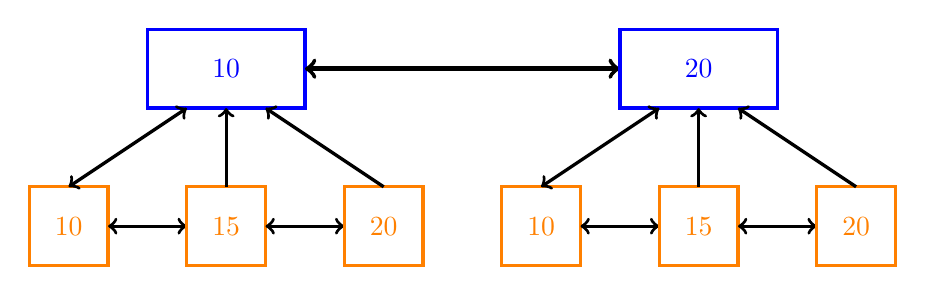
\begin{tikzpicture}
\draw[blue, very thick] (1.5,0) rectangle (3.5,1) node[pos=.5]{10};
\draw[ultra thick, <->] (3.5,0.5) -- (7.5,0.5);
\draw[blue, very thick] (7.5,0) rectangle (9.5,1) node[pos=.5]{20};

\draw[orange, very thick] (0, -2) rectangle (1,-1) node[pos=.5]{10};
\draw[very thick, <->] (0.5,-1) -- (2,0);
\draw[very thick, <->] (1,-1.5) -- (2,-1.5);
\draw[orange, very thick] (2, -2) rectangle (3,-1) node[pos=.5]{15};
\draw[very thick, ->] (2.5,-1) -- (2.5,0);
\draw[very thick, <->] (3,-1.5) -- (4,-1.5);
\draw[orange, very thick] (4, -2) rectangle (5,-1) node[pos=.5]{20};
\draw[very thick, ->] (4.5,-1) -- (3,0);

\draw[orange, very thick] (6, -2) rectangle (7,-1) node[pos=.5]{10};
\draw[very thick, <->] (6.5,-1) -- (8,0);
\draw[very thick, <->] (7,-1.5) -- (8,-1.5);
\draw[orange, very thick] (8,-2) rectangle (9,-1) node[pos=.5]{15};
\draw[very thick, ->] (8.5,-1) -- (8.5,0);
\draw[very thick, <->] (9,-1.5) -- (10,-1.5);
\draw[orange, very thick] (10, -2) rectangle (11,-1) node[pos=.5]{20};
\draw[very thick, ->] (10.5,-1) -- (9,0);

\end{tikzpicture}
\caption{An Order Maintenance data structure. The blue node represent the higher level doubly linked list, and each node store a lower level doubly linked list, denoted by the orange node. Lower level node also store a pointer to the higher level node. Each node additionally hold an unsigned integer, label, such that inside a single list the node earlier have a strictly smaller label then the node later.}
\label{fig:om}
\end{figure}

Concretely, the timestamp for each dirty bit
  is now represented by a pointer to the lower-level OM object.
Priority queue elements are a node pointer,
  an enumeration naming the dirty bit,
  and a pointer to the OM node,
  padded to a total of 16 bytes to align with cache lines.
To compare two timestamps, both pointers must be dereferenced
  to access the two lower-level OM objects.
The associated higher-level OM objects must also be accessed.
In the typical case, where the priority queue remains small,
  all of these OM objects in the priority queue
  are already in cache,
  so ``pops'' have no additional cache misses,
  while ``pushes'' add one, for the new element OM cell.
In total, all the priority queue and order maintenance operations
  thus add the equivalent of 3--5~L2~cache misses in latency,
  about 100--200 cycles.
Since recomputing a field, accessing neighbors' fields,
  and setting neighbors' dirty bits can itself take hundreds of cycles,
  Spineless Traversal's overhead is fairly small.

\subsection{Subtree Insertion}
\label{sec:tree-insertion}

Bulk insertions into the layout tree
  are common in ``lazy loading'' patterns:
  a ``shell'' web page loads first and shows a loading indicator;
  then the ``content'' loads and is inserted a large subtree,
  replacing the loading indicator.
This pattern is encouraged by frameworks like React,
  and can occur in several stages, with a ``shell''
  first inserting ``subshells'' which
  themselves load subcomponents in turn.
Efficiently handling these bulk insertions
  requires special care in Spineless Traversal,
  as bulk insertions are typically responsible
  for Spineless Traversal's worst performance
  relative to Double Dirty Bit.

The basic issue is that in a fresh subtree being inserted into the page,
  every field needs to be computed
  and every OM object needs to be initialized,
  without causing the priority queue itself to grow large.
Our solution adds these ``initialization passes''
  as special elements in the priority queue:
  besides $(v, n)$ pairs for a dirty field $v$ on node $n$,
  an element can also be $(p, r)$,
  a pass $p$ that needs to initialize the entire subtree rooted at $r$.
The timestamp for such a special element
  is just after the last field assigned by $p$
  in $T$'s previous sibling or parent.%
\footnote{
  An edge case is inserting a subtree into
    a subtree that itself has not yet been laid out.
  In this case no further actions need to be taken,
    since both subtrees will be visited together.}

When one of these $(p, r)$ elements is popped from the queue,
  the pass $p$ is performed on the whole subtree under $r$,
  creating all necessary order maintenance nodes
  and computing all fields assigned by $p$.
Since all data accesses are local,
  no existing nodes will refer to any newly-inserted node
  except the root node,
  so no nodes need to be dirtied when running $p$ on the subtree.
This means that, when initializing a subtree,
  no priority queue operations or dirty bit propagations
  need to be performed,
  which makes subtree insertion faster.
However, order maintenance objects still need to be created 
  for every node in the subtree,
  so Spineless Traversal is still
  typically slower than Double Dirty Bit for subtree insertion.

When deleting a subtree,
  some nodes in the subtree may
  already be in the priority queue,
  like when a subtree is inserted and then deleted.
To avoid unnecessary recomputation,
  we add a ``deleted'' bit to each node
  and skip recomputing fields on deleted node.
